\chapter{Theoretical background}
\section{Artificial neural networks}
An artificial neural network is a computing system inspired by the neural structure of the biological brain and its way of processing information. Such structure is able to ``learn'' how to solve certain problems or recognize patterns without being pre-programmed with rules how to do it. Artificial neural networks are main tool used in  deep learning, which is part of bigger family of machine learning \cite{deep_learning_bib}.

\begin{figure}[H]
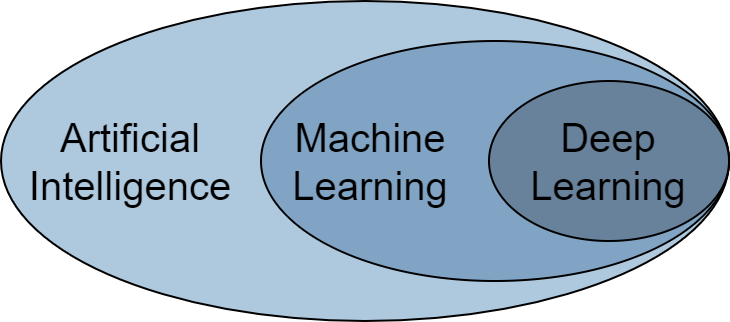
\includegraphics[width=8cm] {deep_learning_chart.png}
\centering
\caption{Deep learning belongingness}
\label{fig:deep_learning_chart}
\end{figure}

Fundamental unit of artificial neural network is so-called ``artificial neuron'' which is a mathematical function modeled after the structure of biological neuron \cite{artificial_neuron_bib}. Such artificial neuron has a number of inputs \(\{x_0, x_1, x_2, ..., x_n\}\) with assigned, separated weights \(\{w_0, w_1, w_2, ..., w_n\}\) for each of them to be multiplied by. In the simplest case, all product are summed and passed to a transfer function \(\varphi\). Additionally a bias value \(b\) is added to the sum of products which allows to shift the activation function up or down. Then the output \(y\) of the neuron is calculated as follows:
%
\begin{equation}
\label{eq:neuron_output}
y = \varphi\left(\sum_{j=0}^{n}x_jw_j\right)
\end{equation}
%
General idea of artificial neuron model is illustrated in figure \ref{fig:artificial_neuron_model}. Typically, neurons are organized into layers which may perform different operations. The output of neurons from one layer is passed to the input of the next layer or might be a part of output vector of whole network. Modern models of artificial neural networks may consist of tens or even hundreds of different layers, on which depends how well given network will cope with certain tasks. Those layers, during process of network training, can adjust theirs weights to produce output values that correctly solve given problem \cite{artificial_neuron_bib} \cite{artificial_neural_networks_bib}.

\begin{figure}[H]
\includegraphics[width=12cm] {artificial_neuron_model.png}
\centering
\caption{Artificial neuron model}
\label{fig:artificial_neuron_model}
\end{figure}

Artificial neural networks have found many, different applications in various fields, in both, academic and business environments. For some time, they are successfully used to solve problems of system identification and control (processes in industrial sector), image classification (medical diagnosis), financial forecasting, face recognition (security), sequence recognition (speech recognition), pattern recognition (data generation) and many more \cite{ann_applications_bib}.

\section{Convolutional neural networks}
Explain how it works, what are main use-cases and so on.

\section{Supervised, unsupervised and semi-supervised training}
Description of both and what are main differences and when to use which.

\section{Haar feature-based cascade classifiers}
\label{Haar feature-based cascade classifiers}
As in section name